\documentclass[journal,12pt,twocolumn]{article}
\usepackage[english]{babel}
\usepackage[letterpaper,top=2cm,bottom=2cm,left=2cm,right=2cm,marginparwidth=1.75cm]{geometry}
\usepackage{multicol}
%\usepackage{amsmath}
\usepackage{graphicx}
%\usepackage{array}
\usepackage{blindtext}
\usepackage[utf8]{inputenc}
\usepackage{watermark}
\usepackage{hyperref}
\usepackage{fancybox}
\usepackage{xcolor}
\newcommand\figref{fig.~\ref}
%\usepackage[colorlinks=true, allcolors=blue]{hyperref}
\usepackage{listings}
\usepackage{float}
\title{FM}
\author{Under guidance of Dr.GVV SHARMA}
\thiswatermark{\centering \put(-50,-105){
\includegraphics[scale=0.7]{iith.png} }}

\begin{document}
\maketitle
\tableofcontents

\section{Abstract}
Finding the bandwidth of an audio signal which is .wav file.

\section{Bandwidth}
Bandwidth can be calculated using various methods. Few of them are: 
\begin{enumerate}
\item The bandwidth of an audio signal can be calculated as the difference between the highest and the lowest frequency components present in the signal.

\item \textbf{Power Spectral Density:}
The bandwidth of a signal can be estimated using its power spectral density by analyzing the frequency range over which a significant portion of the power of the signal is concentrated.

\item \textbf{Half Power Bandwidth:}
The method involves finding the frequency range over which the PSD of the signal is greater than or equal to half of the total power of the signal. This frequency range is known as the half-power bandwidth.

\end{enumerate}
\section{Steps to calculate bandwidth}
\begin{enumerate}

\item \textbf{Loading Audio file:}
We begin by loading the audio file using the wavfile.read() function from the scipy.io.wavfile module. This returns the sampling frequency and the audio data as a numpy array.

\item \textbf{Computing the Fourier Transform:}
	The Fourier transform of the audio signal using the numpy.fft.fft() function. This transforms the audio data from the time domain to the frequency domain.
	
\item \textbf{Calculating Power Spectral Density: }
We calculate the power spectral density (PSD) of the signal by taking the absolute value of the FFT and squaring it.

\item \textbf{Calculating frequency range:}
We also calculate the frequency range using NumPy's \textbf{fftfreq} function, with the sampling interval set to \textbf{1/sample\_rate} to account for the sample rate of the audio file.

\item Finally, we find the frequency range with significant power by applying a mask to the PSD and computing the minimum and maximum frequencies. The bandwidth is simply the difference between these frequencies.we obtain the bandwidth of the audio as 2 khz.
\end{enumerate}
\newpage
Fig. 1 shows the audio spectrum
\begin{figure}[h]
    \centering
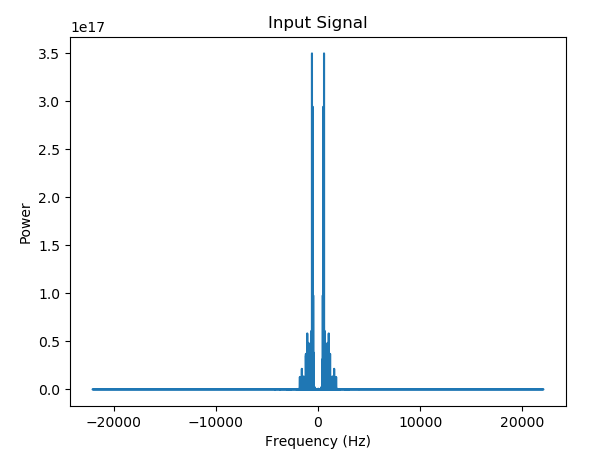
\includegraphics[scale=0.4]{input_spectrum.png} 
    \label{fig:my_label}
    \caption{Spectrum of audio signal}
\end{figure}\\
The below python code computes bandwidth of the input audio file:
   
    \fbox{\parbox{6cm}{\href{https://github.com/NavyaValmeekam/FM/blob/main/FM/codes/bandwidth_audio.py}{/FM/codes/bandwidth$\_$audio.py}}}

\section{Modulation}
\begin{equation}
 c(t) = A_c \cos(2 \pi F_c t )
 \label{eq:carrier_signal} 
 \end{equation}
 Above equation shows the mathematical expression for a carrier signal with amplitude $A_c$, frequency $F_c$. 
 \vspace{1cm}
 \newline
The frequency modulation is applied to the sound signal using the formula
 \begin{equation}
 s(t) = A_c \cos \left(2 \pi F_c t +2\pi K_{f} \int_{0}^t m(\tau) d\tau \right) 
 \end{equation}
where $A_c$ is the amplitude of the carrier signal, $F_c$ is the frequency of the carrier signal, $m(t)$ is the modulating signal, $K_{f}$ is the frequency sensitivity constant of the modulating signal.\\
Fig. 2 shows fm spectrum.
\vspace{4cm}
\\
\begin{figure}
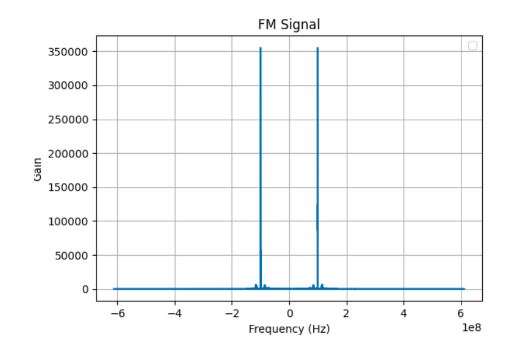
\includegraphics[scale=0.5]{fm_signal.png} 
\label{fig:fm_spectrum}
\caption{FM spectrum}
\end{figure}
The bandwidth of the FM signal generated using a carrier frequency of 100 MHz and frequency sensitivity of 25 kHz is approximately 7 kHz. This was calculated by finding the spectral density of the FM signal using the Fourier transform.\\
The below python code computes bandwidth of the FM signal:
  
    \vspace{0.5cm}
    \fbox{\parbox{6cm}{\href{https://github.com/NavyaValmeekam/FM/blob/main/FM/codes/Modulation.py}{/FM/codes/Modulation.py}}}
    \vspace{0.5cm}
    \\
\begin{figure}
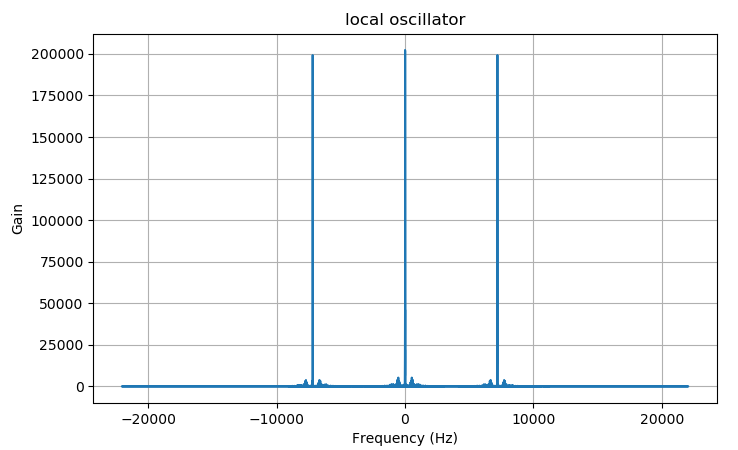
\includegraphics[scale=0.35]{local_oscillator.png}
\label{fig:Local_Oscillator} 
\caption{Local Oscillator Output}
\end{figure} 
\section{Demodulation}
FM signal is multiplied with local oscillator.
Fig. 3 shows the output of it\\
 \begin{equation}
 Y=s(t) \cos(2 \pi F_c t )
 \label{eq:carrier_signal} 
 \end{equation}
\newline
\textbf{Low Pass Filter:}\\
low-pass filter removes the higher-frequency components of the DSB-SC signal, leaving only the sum frequency component (i.e., the FM signal) in the output.\\
Butterworth filter with order 6 and cutoff frequency 3khz gives the filtered FM signal.\\
Fig. 4 shows the Filtered FM signal
\newline
\begin{figure}
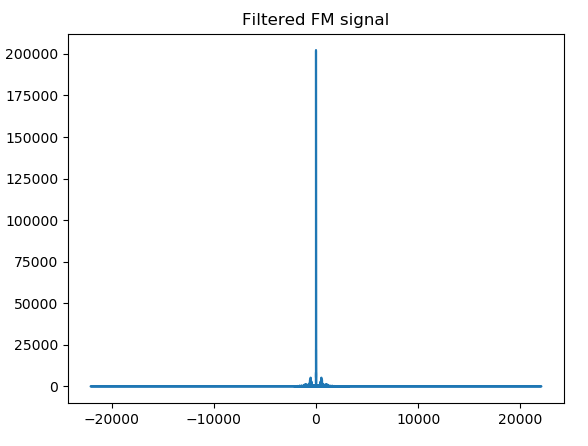
\includegraphics[scale=0.35]{lpf.png} 
\label{fig:Filtered_FM}
\caption{Filtered FM signal}
\end{figure}
\begin{figure}
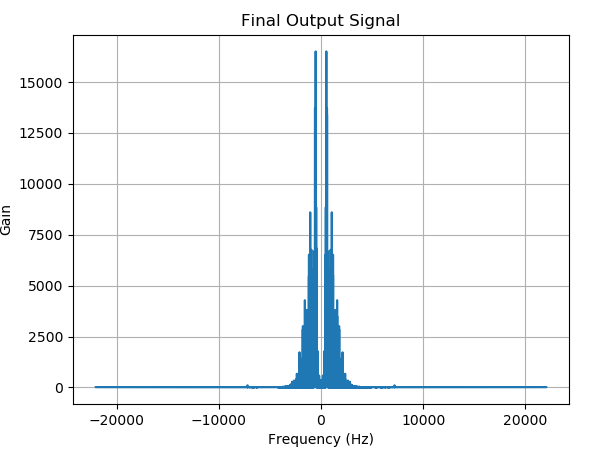
\includegraphics[scale=0.35]{final_output.png} 
\label{fig:Final_Output}
\caption{final output signal}
\end{figure}\\
Cos inverse is applied and differentiated to extract message signal.\\
Fig. 5 shows the final output signal.
\\
\begin{figure}
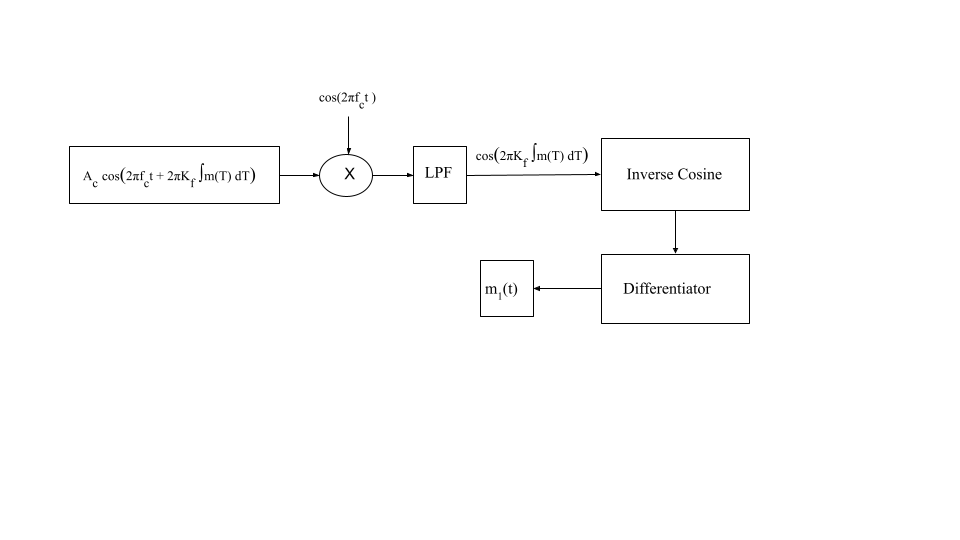
\includegraphics[scale=0.37]{fm block diagram.png} 
\label{fig:Block_diagram}
\caption{Block diagram}
\end{figure}
The below python code generates the demodulated signal:
  
    \vspace{0.5cm}
    \fbox{\parbox{6cm}{\href{https://github.com/NavyaValmeekam/FM/blob/main/FM/codes/fm.py}{/FM/codes/fm.py}}}
\end{document}
